\section{Related Work}
\label{sec:formatting}

We have summarized research work on different aspects of UVDT.

\textbf{Vehicle Detection.}
UVDT mainly uses LiDAR and cameras for vehicle object detection.
Several recent studies have explored the fusion of LiDAR and camera data for vehicle detection,demonstrating significant improvements in both accuracy and robustness. 
For instance, MVDNet (2018) utilizes a multi-view fusion approach, where LiDAR point clouds are projected to different views (such as bird’s-eye view and front view) and matched with camera images, combining depth information from LiDAR and texture information from the camera. 
This method improves detection performance, especially in complex environments\cite{Alpher22h}. 
Building on this, PointPillars introduces a fast encoder for LiDAR data, using a grid-based encoding approach that could potentially be integrated with camera data in future fusion methods to enhance detection speed and efficiency\cite{Alpher19}.
Another study combines LiDAR and camera data by feeding them into separate convolutional neural networks, where the features extracted from both modalities are fused to perform object detection\cite{Alpher20e}. 
This approach has shown significant improvements in detection performance, particularly in dynamic environments with occlusions or sparse LiDAR data.
Lastly, ST-MVDNet introduces a self-training framework using a teacher-student mutual learning mechanism, where the teacher network is trained on the fused LiDAR and camera data, while the student network is exposed to strong data augmentation simulating missing sensor modalities\cite{Alpher22f}. 

This approach enhances the model’s robustness against sensor failures by ensuring consistency between the teacher and student models, allowing the system to better handle missing or noisy data during inference.
These methods collectively highlight the importance of sensor fusion and advanced learning techniques in achieving robust and accurate vehicle detection, even in challenging conditions.
We use the PointPillars deep learning method which has shown good performance.

\textbf{Multi Camera Multi-target Tracking.}
Specker and his team proposed an online multi-camera multi-target tracking method (OCMCTrack), which dynamically optimizes cross-camera target association through an innovative Corrective Matching Cascade strategy, significantly improving tracking accuracy and ID consistency in complex scenarios while ensuring real-time processing\cite{Alpher24e}.
Shim and his team proposes a robust multi-target multi-camera vehicle tracking system designed for city-scale traffic management, addressing challenges like occlusion and cross-camera identity consistency by integrating spatial-temporal constraints and deep feature fusion to enable real-time vehicle monitoring and behavior analysis across urban camera networks\cite{Alpher21e}.
Most existing algorithms, with a few exceptions, can be seen as special cases of the multi-modal fusion problem. 
These methods organize the input data using a graph structure, where edges represent relationships between modalities, and nodes represent different targets or states. 
Algorithms that can be solved in polynomial time typically handle specific modalities or time-continuous edges, with some also utilizing maximum flow or matching algorithms. 
Methods that leverage global information (beyond just time continuity or modality constraints) can significantly improve performance, but they are usually NP-hard due to the involvement of combinatorial optimization. 
In some cases, marginal terms or local constraints are added to ensure completeness. 
To enhance model expressiveness, some studies have employed higher-order relations, although the gains diminish significantly as complexity increases. 
Joint optimization and iterative optimization strategies have also been widely used to improve performance.
We use Joint Integrated Probabilistic Data Association (JIPDA), which combines data from multiple sensors and optimizes probabilistic associations to effectively handle data uncertainty and missing information in target tracking, improving tracking accuracy and robustness in complex environments.


\textbf{Vehicle Reidentification.}
Bing and his team proposed a part-based regularization method, which enhances the accuracy of vehicle re-identification by detecting local parts of vehicles, such as lights and wheels\cite{Alpher19b}. 
Zheng and his colleagues introduced a large-scale vehicle re-identification dataset named VehicleNet and proposed a multi-task learning framework that combines vehicle re-identification and vehicle attribute recognition tasks, improving the model's generalization capability\cite{Alpher20f}. 
P and the research team proposed a dual-path model that integrates global and local features and incorporates an adaptive attention mechanism to enhance the accuracy of vehicle re-identification\cite{Alpher19c}.

The most advanced technologies in the field of vehicle re-identification currently include the combination of deep convolutional neural networks (CNN) for feature extraction and metric learning\cite{Alpher20g}, particularly with the integration of cross-view and cross-domain learning techniques, the use of Generative Adversarial Networks (GAN) for image enhancement\cite{Alpher21d}, and the fusion of multi-sensor data (such as cameras, radar, and LiDAR) to improve the model's robustness and accuracy in complex environments\cite{Alpher22g}.

We designed a ResNet-50 network for vehicle re-identification by drawing inspiration from Re-ID.
The network is capable of performing this task effectively.

\begin{figure*}[t]
	\centering
	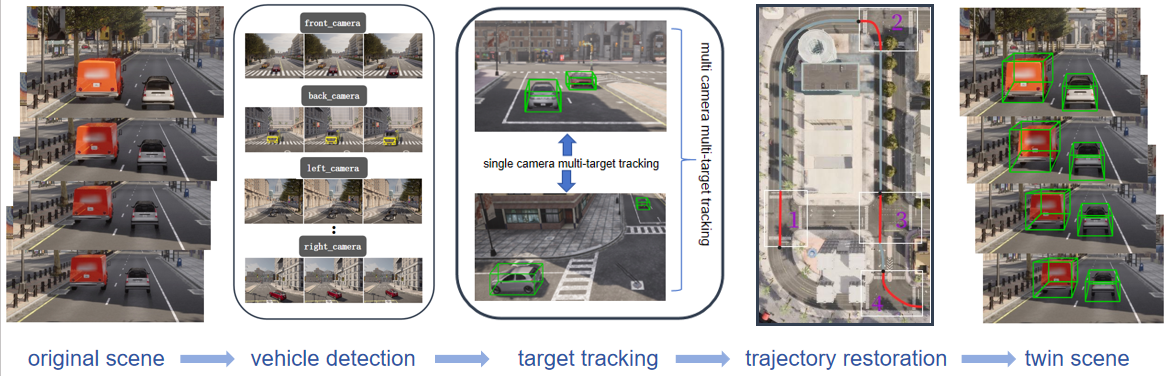
\includegraphics[width=\textwidth]{picture/picture2.png} 
	\caption{Given the original scene, cameras and radar detect vehicles, and the tracker performs single-camera multi-target tracking and multi-camera multi-target tracking. The data obtained from tracking is used for trajectory reconstruction, and finally, a digital twin is created to replicate the traffic scenario.}
	\label{fig:example}
\end{figure*}

\textbf{Twin.}
After obtaining all the data, we will proceed with vehicle control. 
Kaleb Ben Naveed et al. proposed a hierarchical reinforcement learning-based method for autonomous driving trajectory planning and control. 
By training a reinforcement learning agent in a simulation environment, this method optimizes the vehicle's control strategy according to environmental changes, achieving efficient trajectory planning and dynamic path adjustment.\cite{Alpher22}
R. Barea et al. proposed a deep reinforcement learning (DRL)-based control method, where an agent is trained in the CARLA simulation platform to autonomously learn and optimize the vehicle's control strategies (such as throttle, brake, and steering) to ensure safe and smooth driving.\cite{Alpher21}
We optimize the trajectories obtained from multi-object tracking using a trajectory smoothing algorithm, enabling the vehicle to turn more smoothly and drive more steadily (reducing bumps and sudden maneuvers) while ensuring precise adherence to the planned path at a lower computational cost. 
Subsequently, the PID control algorithm is employed to control the vehicle, guiding it to follow the optimized trajectory and achieve final trajectory-tracking synchronization.